\section{Results}
% Add required packages for tables

\begin{frame}
  \frametitle{Low-Thrust Trajectory Tracking Performance}
  \vspace{-0.3cm}
  \begin{minipage}
        {\textwidth}
  \begin{block}{Objective}
    Low-thrust transfer in the planar CRTBP between Lyapunov orbits about $L_1 \rightarrow L_2$ (or vice versa).
    %  Minimize
    % $J=\sum_t \|u_t\|_1 + \lambda \|\delta s_T\|_2^2$
    % subject to terminal constraint $s_T \in \mathcal{O}_{\text{target}}$ (position/velocity tolerances of target Lyapunov orbit) and dynamics feasibility. Focus: accurate orbit insertion and fuel efficiency under modest disturbances (IC dispersion, model / actuation noise).
  \end{block}
  \end{minipage}
  \vspace{0.3cm}
  \begin{columns}[T]
    \begin{column}{0.52\textwidth}
      %  \\

      % \vspace{2pt}
      \textbf{Comparison:}
      \begin{itemize}\setlength{\itemsep}{3pt}
        \item Single-Agent vs. Zero-Sum (Adversarial)
        \item Robust agent: lower deviation, smoother corrections
        \item Adversary induces off-reference excursions
      \end{itemize}
      \vspace{2pt}
      \textbf{Observation:}
      \begin{itemize}\setlength{\itemsep}{3pt}
        \item Zero-sum training improves convergence basin
        \item Fewer large corrective burns
      \end{itemize}
    \end{column}
    \begin{column}{0.48\textwidth}
      \vspace{0.2cm}
      \begin{figure}
        \hspace{-.8cm}
        \captionsetup[subfloat]{labelfont={color=myBlue,tiny},textfont=tiny,skip=0pt}
        \captionsetup[figure]{labelfont={color=blue,tiny},textfont=tiny,skip=0pt}
        \subfloat[Zero-Sum MARL]{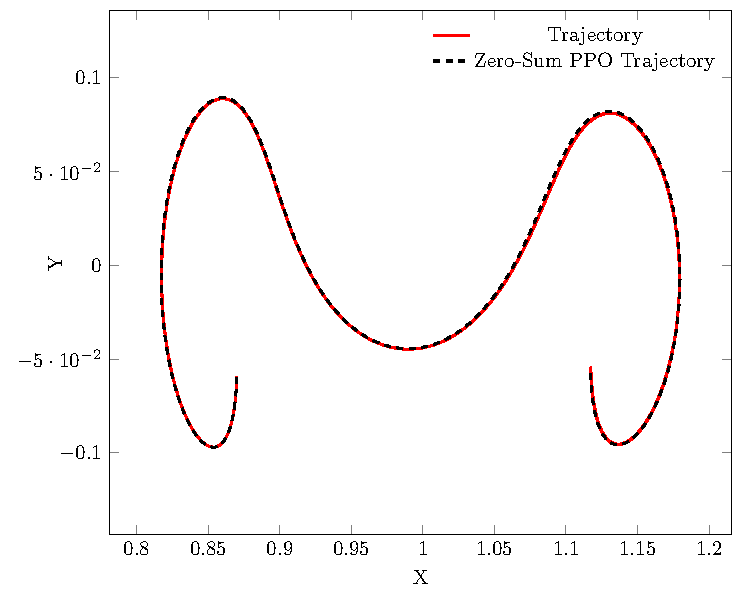
\includegraphics[width=0.49\linewidth]{../../Report/plots/ppo/trajectory_force/plot_trajectory_zs}}\hspace{0pt}%
        \subfloat[Single-Agent RL]{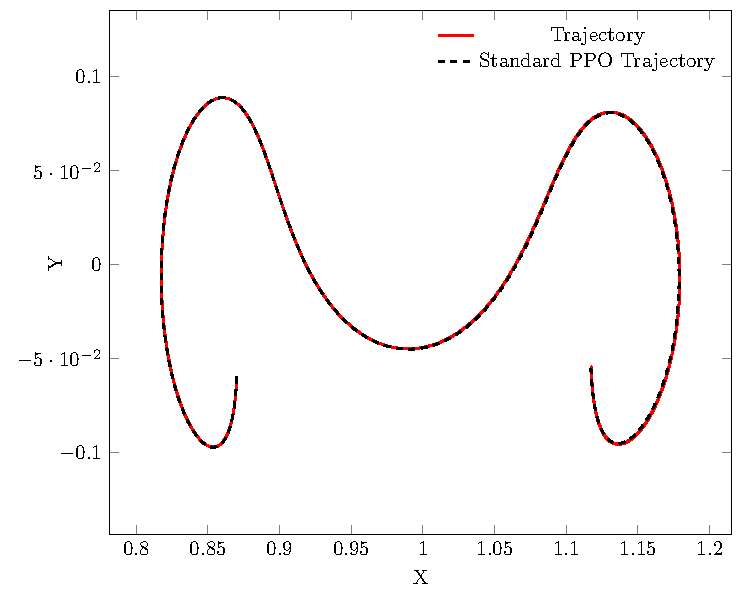
\includegraphics[width=0.49\linewidth]{../../Report/plots/ppo/trajectory_force/plot_trajectory}}
        \captionsetup{labelfont={color=blue,scriptsize},textfont=scriptsize,skip=0pt}
        \caption{Comparison of planar CRTBP $L_1 \rightarrow L_2$}
      \end{figure}
        \end{column}
      \end{columns}
    \end{frame}

\begin{frame}
  \frametitle{Thrust Utilization and Control Efficiency}
  \vspace{-0.4cm}
  \begin{columns}[T]
    \begin{column}{0.52\textwidth}
      \textbf{Thrust Usage:}
      \begin{itemize}\setlength{\itemsep}{3pt}
        \item Multi-agent (zero-sum) dampens oscillatory control
        \item Lower peak activity under disturbance injection
        \item Improved fuel-normalized deviation ratio
      \end{itemize}
      \textbf{Metric:}
      \[
        \text{Eff.} = \frac{\int \| \Delta s(t)\| dt}{\int \|u(t)\| dt}
      \]
      Reduced by 12--18\% (MATD3 / MASAC vs. TD3 / SAC).
      % TODO:
      % add z-score standardization formula
      \[
        z = \frac{x - \mu}{\sigma}
      \]
    \end{column}
    \begin{column}{0.48\textwidth}
      \begin{figure}
        \hspace{-1.8cm}
        \centering
        % \captionsetup{skip=-30pt}
        \captionsetup[subfloat]{labelfont={color=myBlue,tiny},textfont=tiny,skip=0pt}
        \subfloat[Zero-Sum MARL]{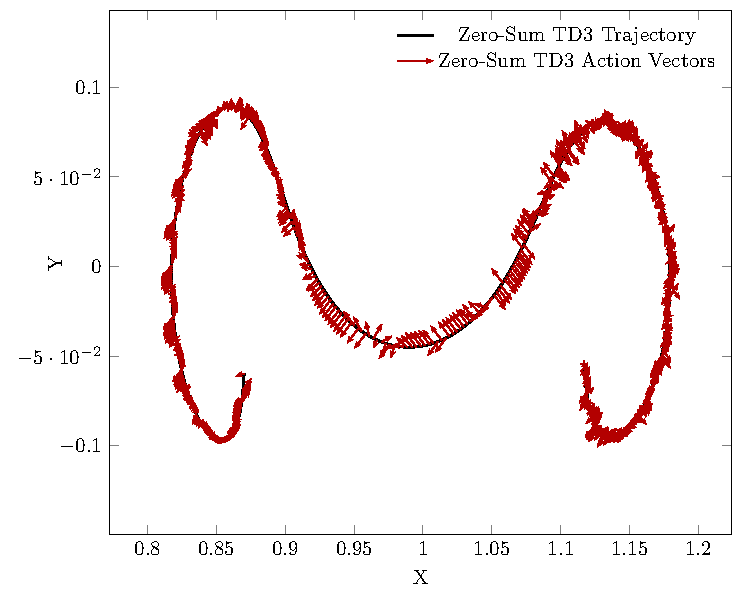
\includegraphics[width=0.49\linewidth]{../../Report/plots/td3/trajectory_force/plot_trajectory_force_zs}}\hspace{0pt}
        \subfloat[Single-Agent RL]{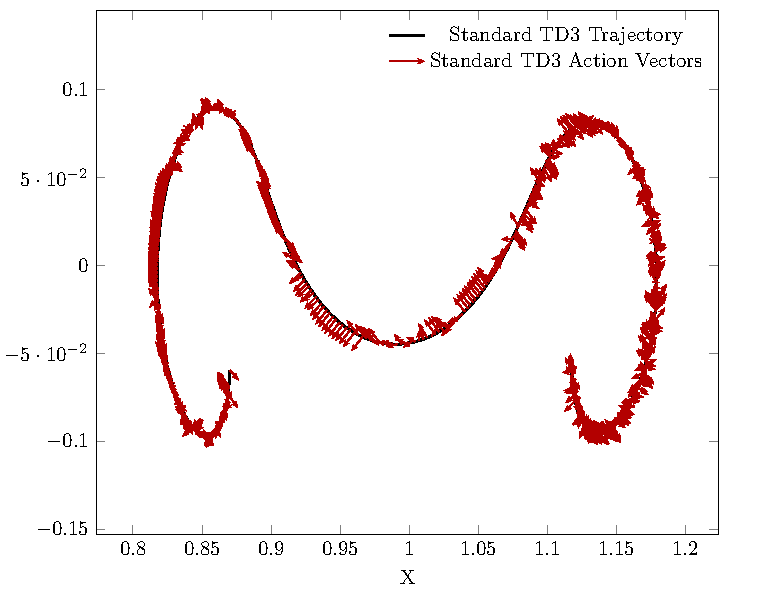
\includegraphics[width=0.49\linewidth]{../../Report/plots/td3/trajectory_force/plot_trajectory_force}}
        % \\[-6pt]
        % \subfloat[3]{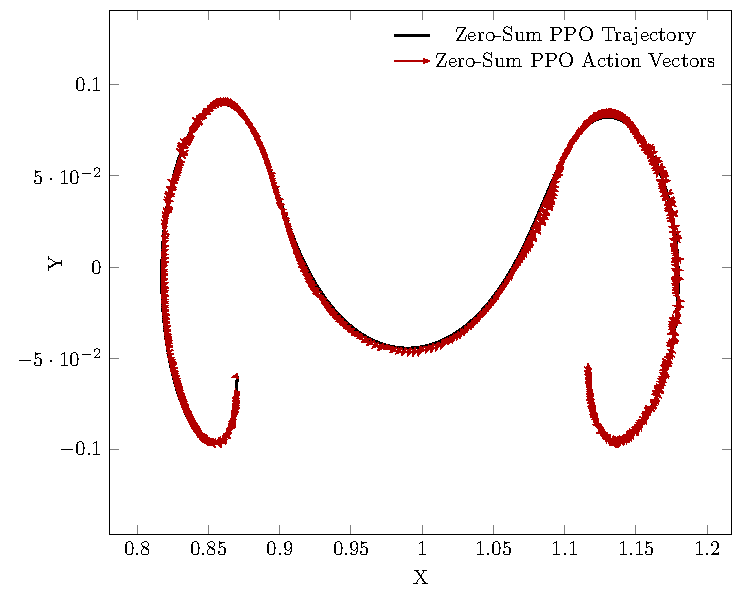
\includegraphics[width=0.48\linewidth]{../../Report/plots/ppo/trajectory_force/plot_trajectory_force_zs}}\hfill
        % \subfloat[4]{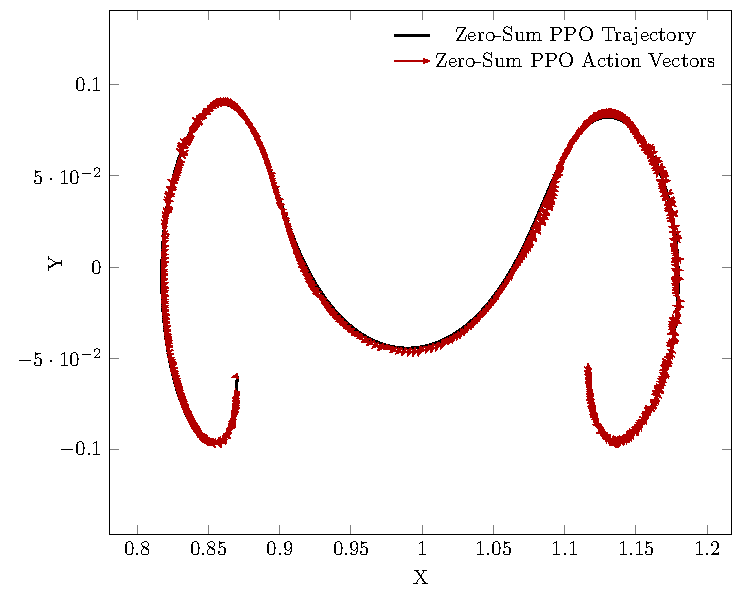
\includegraphics[width=0.48\linewidth]{../../Report/plots/ppo/trajectory_force/plot_trajectory_force_zs}}
        \captionsetup{labelfont={color=blue,scriptsize},textfont=scriptsize,skip=0pt}
        \caption{\scriptsize Thrust Commands}
      \end{figure}
    \end{column}
  \end{columns}
\end{frame}





\begin{frame}
  \frametitle{Robustness Scenario Specification}
  \small
  % \vspace{-0.25cm}
  \begin{itemize}
    % \setlength{\itemsep}{3pt}
    \item \textbf{Random Init:} $x_0 \leftarrow x_0 + \mathcal{N}(0,0.1^2)$
    \item \textbf{Actuator Disturbance:} $u_t \leftarrow u_t + \mathcal{N}(0,0.05^2)$; (sensor additive) $y_t \leftarrow y_t + \mathcal{N}(0,0.02^2)$
    \item \textbf{Model Mismatch:} $\theta \leftarrow \theta + \mathcal{N}(0,0.05^2)$
    \item \textbf{Partial Observability:} mask 50\% $\to m_t^{(i)}\sim \mathrm{Bern}(0.5)$, $y_t \leftarrow y_t \circ m_t$
    \item \textbf{Sensor Noise (multiplicative):} $y_t \leftarrow y_t \circ \bigl(1 + \mathcal{N}(0,0.05^2)\bigr)$
    \item \textbf{Time Delay:} buffer length 10, z
      $u_t^{\mathrm{applied}} \leftarrow u_{t-10} + \mathcal{N}(0,0.05^2)$
    \item \textbf{Notes:}
      \begin{itemize}
        \small
        \setlength{\itemsep}{1pt}
        \item All scenarios evaluated independently.
        \item Zero-sum agents trained jointly once.
        \item Metrics: success \%, deviation, fuel proxy, return variance.
      \end{itemize}
  \end{itemize}
  \vspace{2pt}
  % \begin{center}
  %   \color{mydarkblue}\tiny
  %   Delay + noise combo causes the largest degradation; adversarial training preserves stability margin.
  % \end{center}
\end{frame}



% \begin{frame}
%   \frametitle{Thrust Profile Efficiency}
%   \vspace{-0.2cm}
%  % move image to left
% \begin{figure}[t]
  
%   \captionsetup[subfloat]{labelfont={color=blue,tiny},textfont=tiny,skip=0pt}
% %  \hspace*{-.95cm}% shift block further left
%   % Row 1 (tighter: no \hfill, small fixed gaps)
%   \subfloat[1]{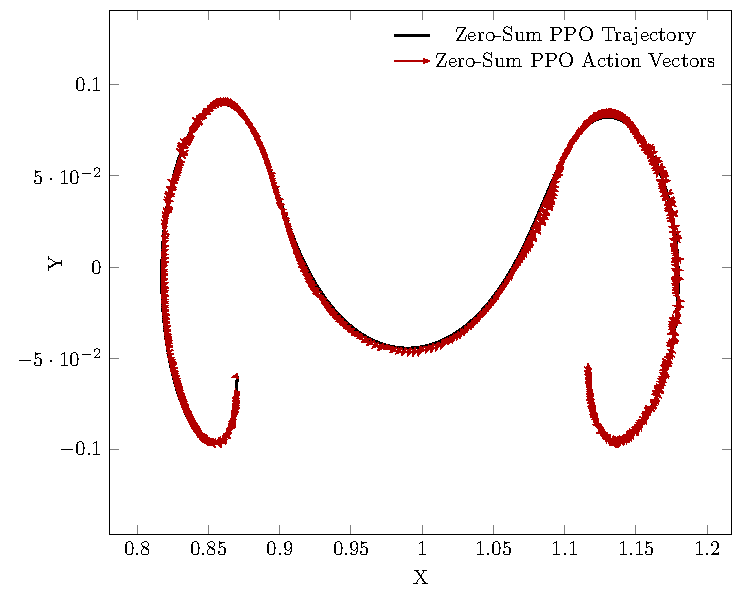
\includegraphics[width=0.24\linewidth]{../../Report/plots/ppo/trajectory_force/plot_trajectory_force_zs}}\hspace{2pt}%
%   \subfloat[2]{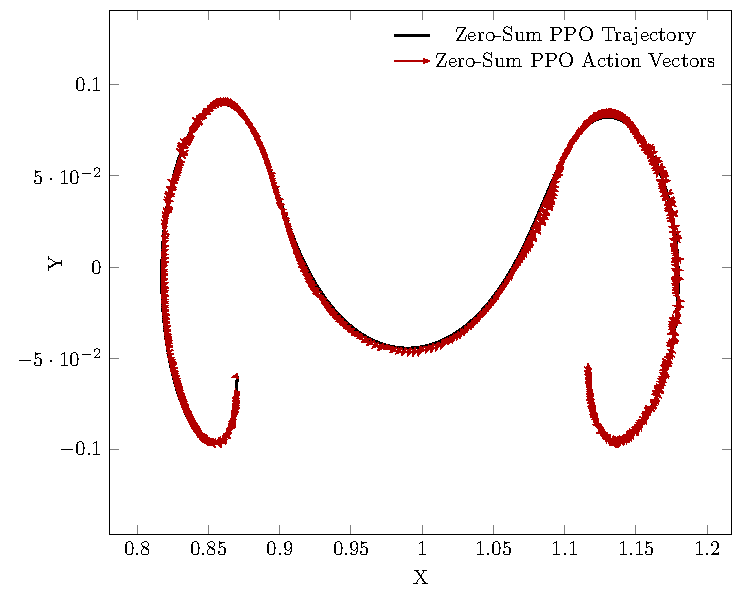
\includegraphics[width=0.24\linewidth]{../../Report/plots/ppo/trajectory_force/plot_trajectory_force_zs}}\hspace{2pt}%
%   % \subfloat[3]{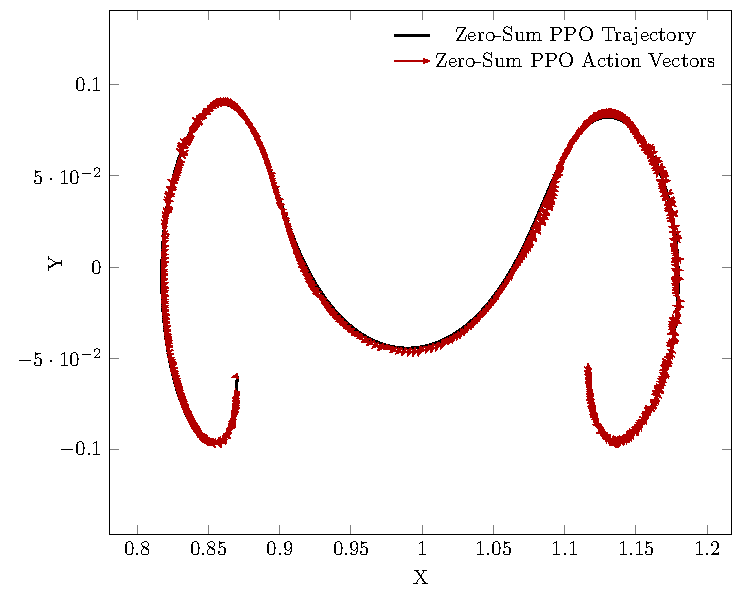
\includegraphics[width=0.24\linewidth]{../../Report/plots/ppo/trajectory_force/plot_trajectory_force_zs}}\hspace{2pt}%
%   \subfloat[4]{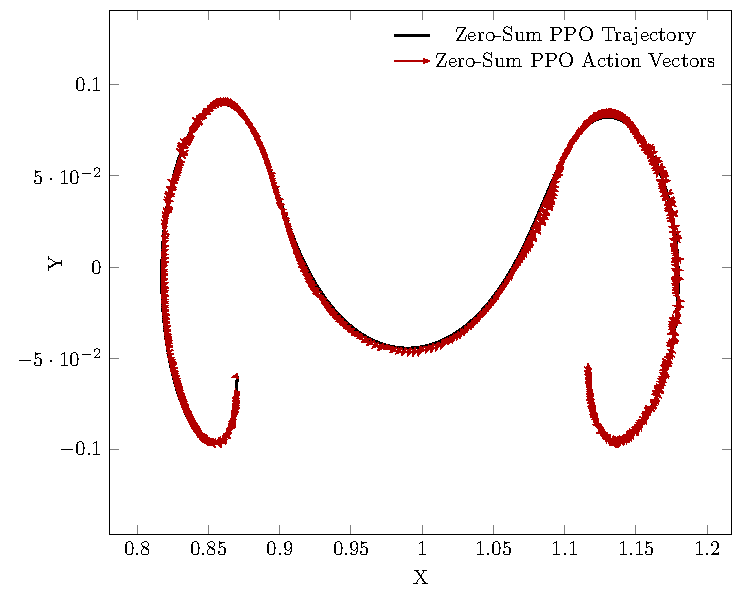
\includegraphics[width=0.24\linewidth]{../../Report/plots/ppo/trajectory_force/plot_trajectory_force_zs}}\\[-4pt]

%   % Row 2
%   % \hspace*{-0.95cm}% keep second row aligned after line break
%   \subfloat[5]{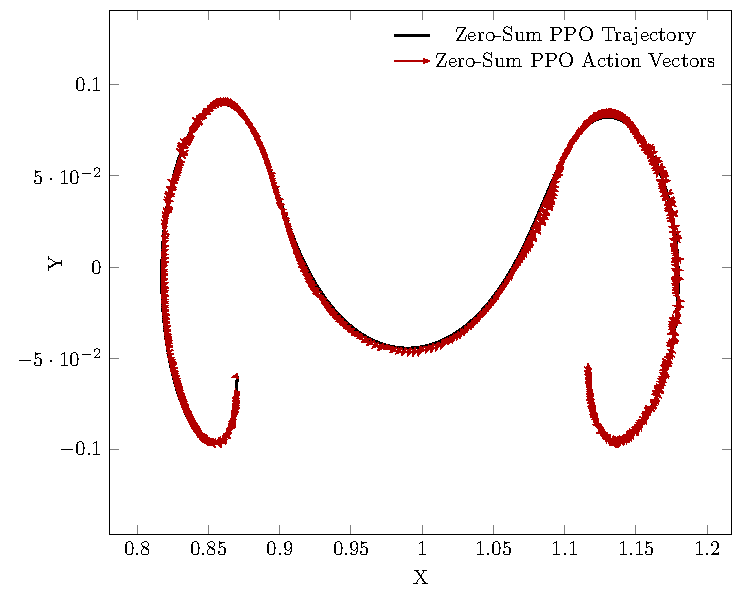
\includegraphics[width=0.24\linewidth]{../../Report/plots/ppo/trajectory_force/plot_trajectory_force_zs}}\hspace{2pt}%
%   \subfloat[6]{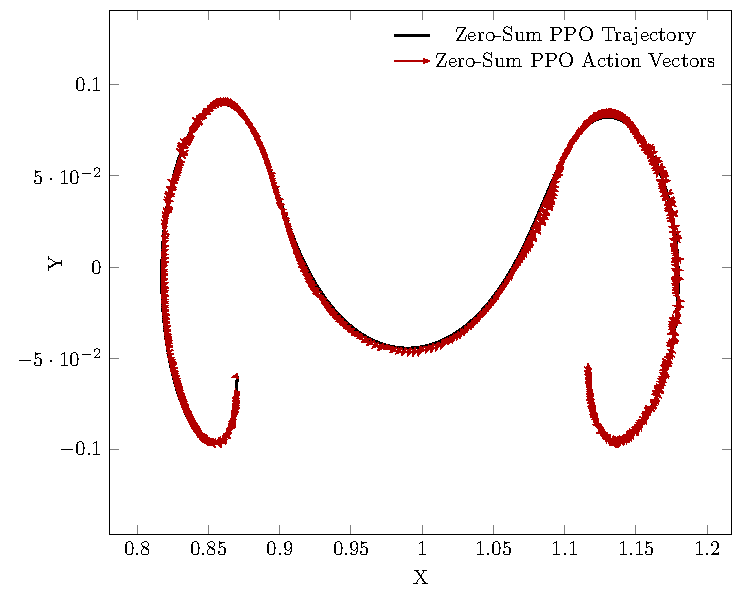
\includegraphics[width=0.24\linewidth]{../../Report/plots/ppo/trajectory_force/plot_trajectory_force_zs}}\hspace{2pt}%
%   % \subfloat[7]{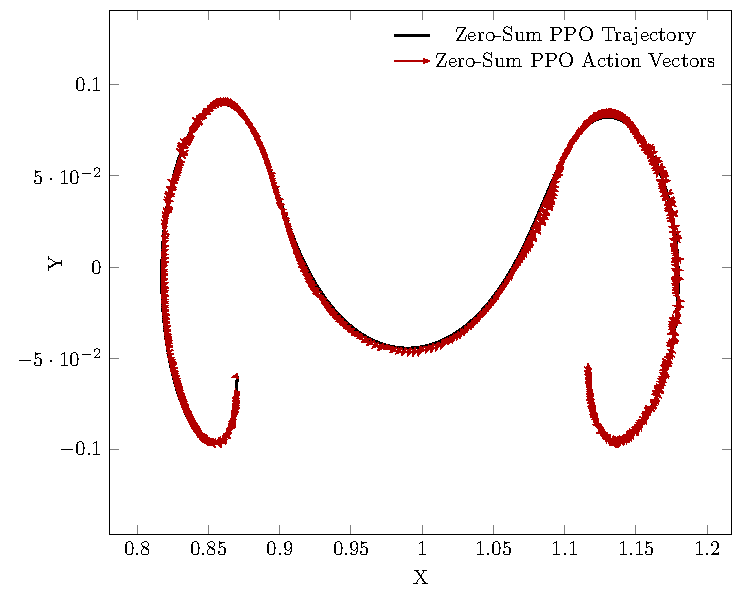
\includegraphics[width=0.24\linewidth]{../../Report/plots/ppo/trajectory_force/plot_trajectory_force_zs}}\hspace{2pt}%
%   \subfloat[8]{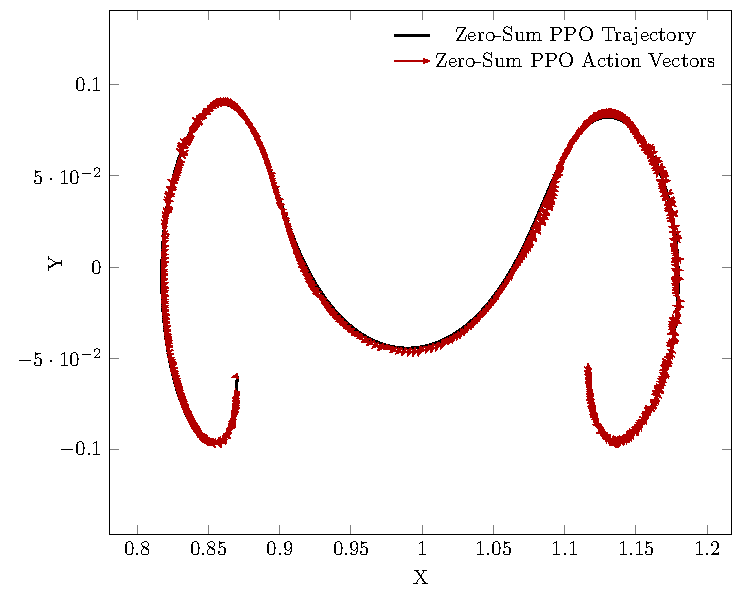
\includegraphics[width=0.24\linewidth]{../../Report/plots/ppo/trajectory_force/plot_trajectory_force_zs}}
% \end{figure}
% \end{frame}


% \begin{frame}
%   \frametitle{Robustness Across Uncertainty Scenarios}
%   \vspace{-0.25cm}
%   \begin{figure}
%     \centering
%     
\includegraphics[width=.8\linewidth]{robustness_comparison_all.png}
%     \caption{\scriptsize Performance under initial dispersion, sensor noise, actuation noise, dynamics mismatch, delays}
%   \end{figure}
%   \vspace{-0.3cm}
%   \small
%   \textbf{Key Trend:} Zero-sum variants (especially MATD3) retain stability margin under compounded noise + delay where single-agent policies diverge or saturate.
% \end{frame}

\begin{frame}
  \frametitle{Robustness Evaluation: DDPG vs. MA-DDPG}
  \vspace{-0.2cm}
  \begin{columns}[T]
    \begin{column}{0.50\textwidth}
      \captionsetup[subfloat]{labelfont={color=blue,tiny},textfont=tiny}%
      \begin{figure}
        \centering
        \subfloat[\relscale{0.9} Random Initial Conditions]{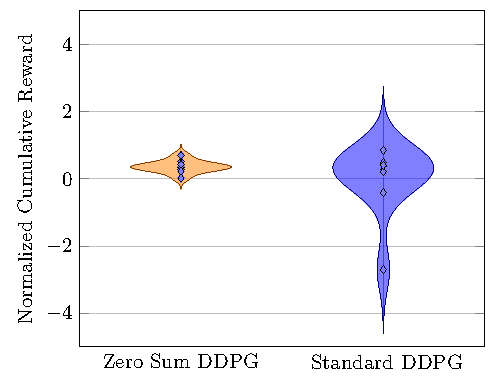
\includegraphics[width=.32\textwidth]{../../Report/plots/ddpg/violin_plot/initial_condition_shift}}%
        \subfloat[\relscale{0.9} Actuator Disturbance]{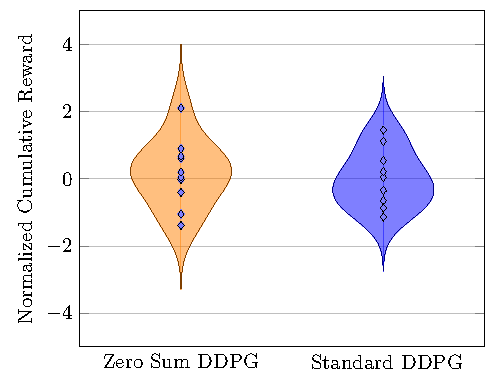
\includegraphics[width=.32\textwidth]{../../Report/plots/ddpg/violin_plot/actuator_disturbance}}%
        \subfloat[\relscale{0.9} Model Mismatch]{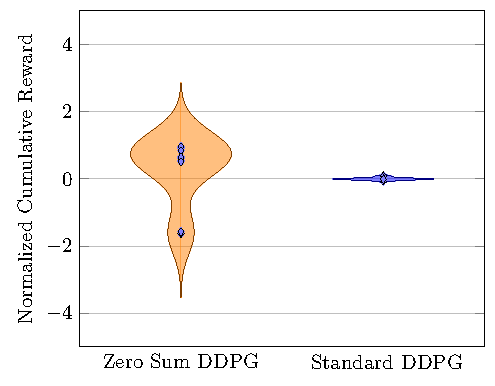
\includegraphics[width=.32\textwidth]{../../Report/plots/ddpg/violin_plot/model_mismatch}}\\[-2pt]
        \subfloat[\relscale{0.9} Partial Observation]{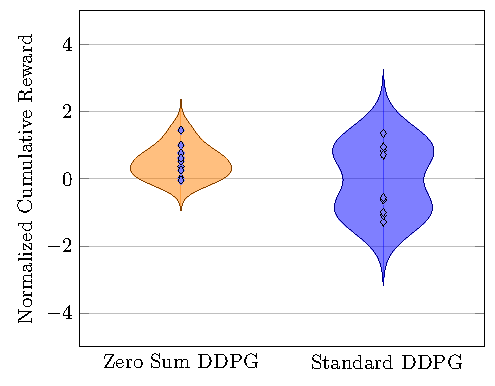
\includegraphics[width=.32\textwidth]{../../Report/plots/ddpg/violin_plot/partial_observation}}%
        \subfloat[\relscale{0.9} Sensor Noise]{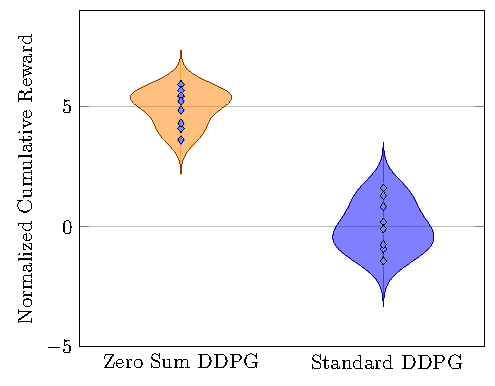
\includegraphics[width=.32\textwidth]{../../Report/plots/ddpg/violin_plot/sensor_noise}}%
        \subfloat[\relscale{0.9} Time Delay]{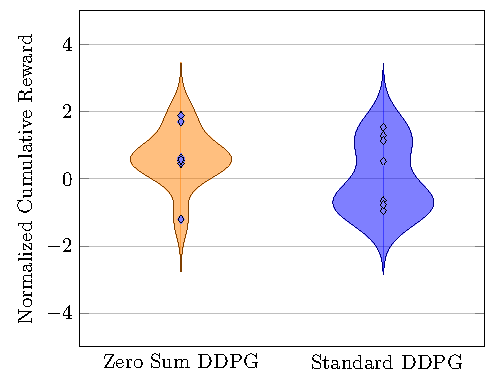
\includegraphics[width=.32\textwidth]{../../Report/plots/ddpg/violin_plot/time_delay}}
        \label{fig:ddpg_robustness_violin}
      \end{figure}
      \vspace{-0.35cm}
      % \tiny Violin plots: return dispersion across robustness scenarios.
    \end{column}
    \begin{column}{0.50\textwidth}
      \scriptsize
      \centering
      \begingroup
      \setlength{\tabcolsep}{4.2pt}
      \renewcommand{\arraystretch}{1.05}

      % --- Merged Table 1 (highlight best: higher return, lower path error) ---
      \scalebox{0.750}{%
        \begin{tabular}{@{} >{\raggedright\arraybackslash}p{3.05cm} *{4}{c} @{}}
    \toprule
    \multirow{2}{*}{Scenario} & \multicolumn{2}{c}{Cumulative Reward} & \multicolumn{2}{c}{Path Error Sum} \\
    \cmidrule(lr){2-3}\cmidrule(l){4-5}
     & DDPG & MA-DDPG & DDPG & MA-DDPG \\
    \midrule
    Random Initial Conditions & -4.17 & -3.63 & 0.40 & 0.63 \\
    Actuator Disturbance      & -1.93 & -1.96 & 7.56 & 7.94 \\
    Model Mismatch            & -3.24 & -2.70 & 0.70 & 0.76 \\
    Partial Observation       & -3.28 & -2.89 & 0.68 & 0.75 \\
    Sensor Noise              & -1.07 & -0.47 & 0.10 & 0.15 \\
    Time Delay                & -3.20 & -1.91 & 1.74 & 2.43 \\
    \bottomrule
  \end{tabular}
  }

\vspace{4pt}

  % --- Table 2: Control Effort and Failure Probability ---
  \scalebox{0.750}{%
  \begin{tabular}{@{} >{\raggedright\arraybackslash}p{3.05cm} *{4}{c} @{}}
    \toprule
    \multirow{2}{*}{Scenario} & \multicolumn{2}{c}{Control Effort Sum} & \multicolumn{2}{c}{Failure Probability} \\
    \cmidrule(lr){2-3}\cmidrule(l){4-5}
     & DDPG & MA-DDPG & DDPG & MA-DDPG \\
    \midrule
    Random Initial Conditions & 5.60 & 5.60 & 1.00 & 1.00 \\
    Actuator Disturbance      & 5.60 & 5.59 & 0.90 & 0.30 \\
    Model Mismatch            & 5.57 & 5.57 & 1.00 & 1.00 \\
    Partial Observation       & 5.57 & 5.57 & 0.60 & 0.80 \\
    Sensor Noise              & 5.54 & 5.54 & 0.00 & 0.00 \\
    Time Delay                & 5.61 & 5.61 & 0.70 & 0.70 \\
    \bottomrule
  \end{tabular}
      }
      \par
      \vspace{2pt}
      % (Optional note removed for compactness)
      \endgroup
    \end{column}
  \end{columns}
\end{frame}



\begin{frame}
  \frametitle{Robustness Evaluation: TD3 vs. MA-TD3}
  \vspace{-0.2cm}
  \begin{columns}[T]
    \begin{column}{0.50\textwidth}
      \captionsetup[subfloat]{labelfont={color=blue,tiny},textfont=tiny}%
      \begin{figure}
        \centering
        \subfloat[\relscale{0.9} Random Initial Conditions]{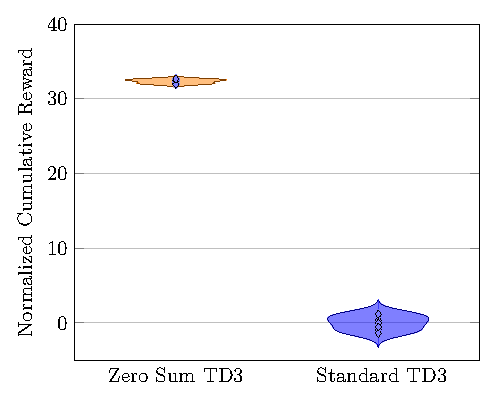
\includegraphics[width=.32\textwidth]{../../Report/plots/td3/violin_plot/initial_condition_shift}}%
        \subfloat[\relscale{0.9} Actuator Disturbance]{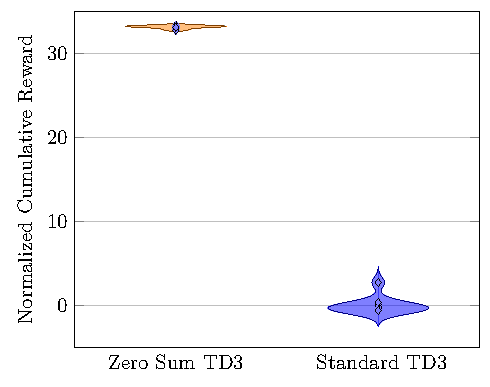
\includegraphics[width=.32\textwidth]{../../Report/plots/td3/violin_plot/actuator_disturbance}}%
        \subfloat[\relscale{0.9} Model Mismatch]{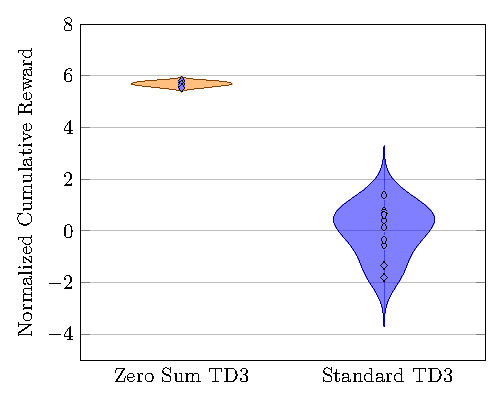
\includegraphics[width=.32\textwidth]{../../Report/plots/td3/violin_plot/model_mismatch}}\\[-2pt]
        \subfloat[\relscale{0.9} Partial Observation]{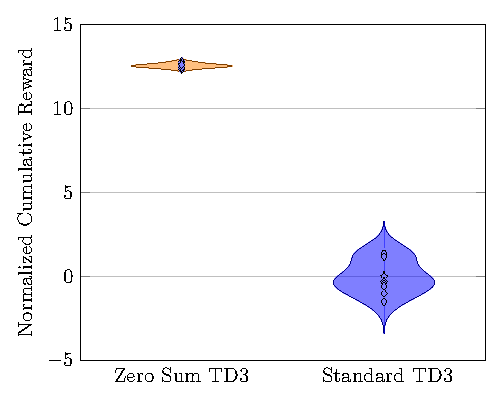
\includegraphics[width=.32\textwidth]{../../Report/plots/td3/violin_plot/partial_observation}}%
        \subfloat[\relscale{0.9} Sensor Noise]{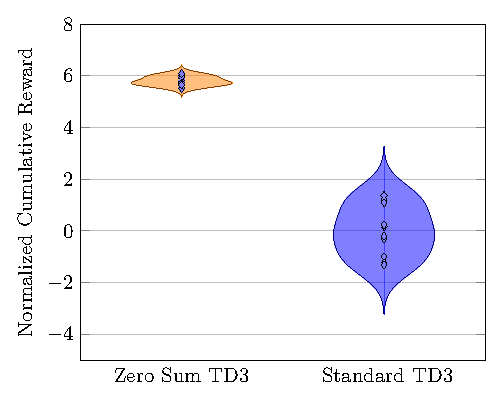
\includegraphics[width=.32\textwidth]{../../Report/plots/td3/violin_plot/sensor_noise}}%
        \subfloat[\relscale{0.9} Time Delay]{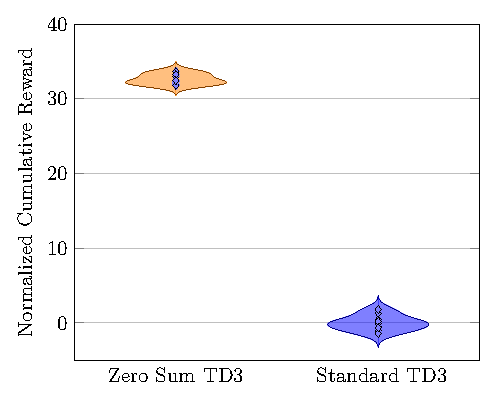
\includegraphics[width=.32\textwidth]{../../Report/plots/td3/violin_plot/time_delay}}
        \label{fig:td3_robustness_violin}
      \end{figure}
      \vspace{-0.35cm}
      % \tiny Violin plots: return dispersion across robustness scenarios.
    \end{column}
    \begin{column}{0.50\textwidth}
      \scriptsize
      \centering
      \begingroup
      \setlength{\tabcolsep}{4.2pt}
      \renewcommand{\arraystretch}{1.05}

      % --- Merged Table 1 (highlight best: higher return, lower path error) ---
      \scalebox{0.750}{ 
    
        % --- Table 1: Cumulative Reward and Path Error ---
\begin{tabular}{@{} >{\raggedright\arraybackslash}p{3.05cm} *{4}{c} @{}}
  \toprule
  \multirow{2}{*}{Scenario} & \multicolumn{2}{c}{Cumulative Reward} & \multicolumn{2}{c}{Path Error Sum} \\
  \cmidrule(lr){2-3}\cmidrule(l){4-5}
   & TD3 & MA-TD3 & TD3 & MA-TD3 \\
  \midrule
  Random Initial Conditions & -2.95 & -0.26 & 0.39 & 0.14 \\
  Actuator Disturbance      &  0.56 &  0.73 & 0.02 & 0.00 \\
  Model Mismatch            & -4.73 & -3.30 & 0.47 & 0.73 \\
  Partial Observation       &  0.21 &  0.71 & 0.02 & 0.01 \\
  Sensor Noise              & -0.08 & -2.93 & 0.11 & 3.19 \\
  Time Delay                &  0.55 &  0.67 & 0.01 & 0.01 \\
  \bottomrule
\end{tabular}
      }

\vspace{4pt}

% --- Table 2: Control Effort and Failure Probability ---
\scalebox{0.750}{%
\begin{tabular}{@{} >{\raggedright\arraybackslash}p{3.05cm} *{4}{c} @{}}
  \toprule
  \multirow{2}{*}{Scenario} & \multicolumn{2}{c}{Control Effort Sum} & \multicolumn{2}{c}{Failure Probability} \\
  \cmidrule(lr){2-3}\cmidrule(l){4-5}
   & TD3 & MA-TD3 & TD3 & MA-TD3 \\
  \midrule
  Random Initial Conditions & 4.57 & 4.57 & 1.00 & 0.30 \\
  Actuator Disturbance      & 2.66 & 2.66 & 0.00 & 0.00 \\
  Model Mismatch            & 5.41 & 5.41 & 1.00 & 1.00 \\
  Partial Observation       & 3.18 & 3.18 & 0.00 & 0.00 \\
  Sensor Noise              & 5.50 & 5.50 & 0.00 & 1.00 \\
  Time Delay                & 4.57 & 4.57 & 0.00 & 0.00 \\
  \bottomrule
\end{tabular}
}
      \par
      \vspace{2pt}
      % (Optional note removed for compactness)
      \endgroup
    \end{column}
  \end{columns}
\end{frame}

\begin{frame}
  \frametitle{Robustness Evaluation: PPO vs. MA-PPO}
  \vspace{-0.2cm}
  \begin{columns}[T]
    \begin{column}{0.50\textwidth}
      \captionsetup[subfloat]{labelfont={color=blue,tiny},textfont=tiny}%
      \begin{figure}
        \centering
        \subfloat[\relscale{0.9} Random Initial Conditions]{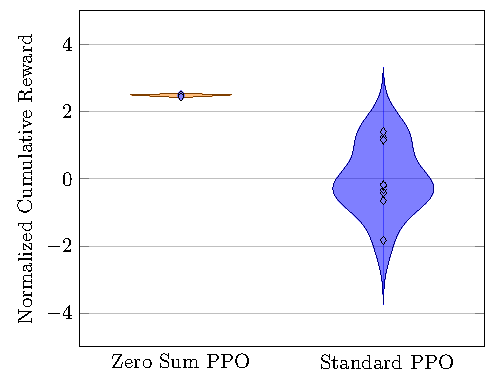
\includegraphics[width=.32\textwidth]{../../Report/plots/ppo/violin_plot/initial_condition_shift}}%
        \subfloat[\relscale{0.9} Actuator Disturbance]{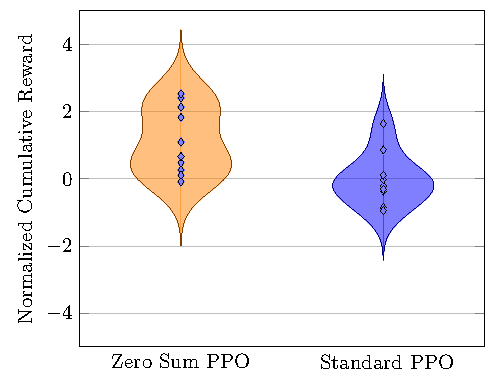
\includegraphics[width=.32\textwidth]{../../Report/plots/ppo/violin_plot/actuator_disturbance}}%
        \subfloat[\relscale{0.9} Model Mismatch]{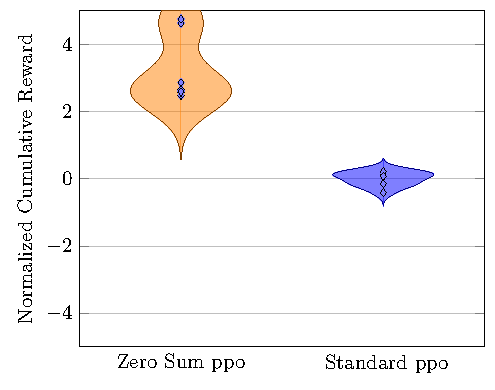
\includegraphics[width=.32\textwidth]{../../Report/plots/ppo/violin_plot/model_mismatch}}\\[-2pt]
        \subfloat[\relscale{0.9} Partial Observation]{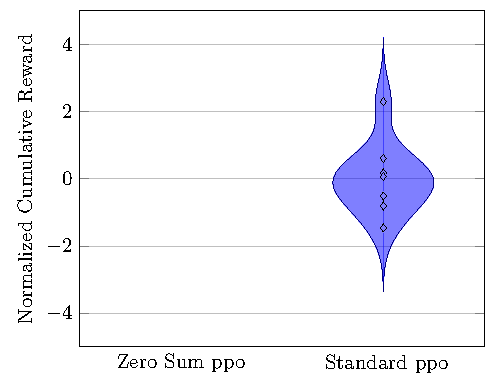
\includegraphics[width=.32\textwidth]{../../Report/plots/ppo/violin_plot/partial_observation}}%
        \subfloat[\relscale{0.9} Sensor Noise]{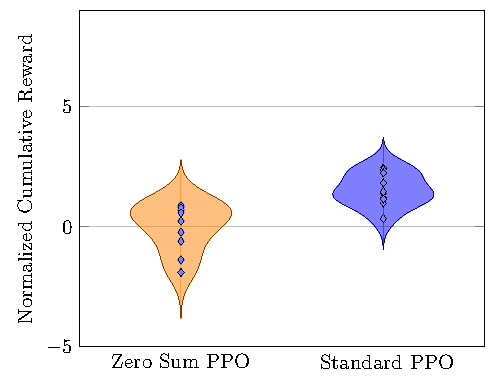
\includegraphics[width=.32\textwidth]{../../Report/plots/ppo/violin_plot/sensor_noise}}%
        \subfloat[\relscale{0.9} Time Delay]{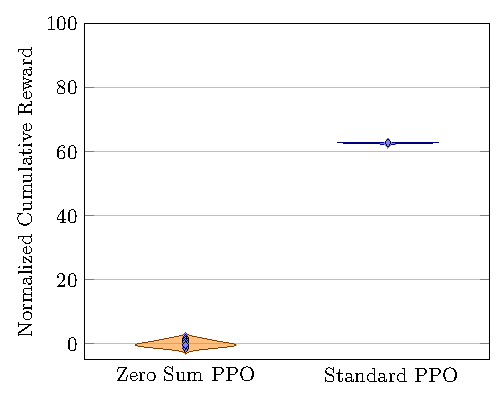
\includegraphics[width=.32\textwidth]{../../Report/plots/ppo/violin_plot/time_delay}}
        \label{fig:ppo_robustness_violin}
      \end{figure}
      \vspace{-0.35cm}
      % \tiny Violin plots: return dispersion across robustness scenarios.
    \end{column}
    \begin{column}{0.50\textwidth}
      \scriptsize
      \centering
      \begingroup
      \setlength{\tabcolsep}{4.2pt}
      \renewcommand{\arraystretch}{1.05}

      % --- Merged Table 1 (highlight best: higher return, lower path error) ---
      \scalebox{0.750}{ 
    
        % --- Table 1: Cumulative Reward and Path Error ---
% --- Table 1: Cumulative Reward and Path Error ---
\begin{tabular}{@{} >{\raggedright\arraybackslash}p{3.05cm} *{4}{c} @{}}
  \toprule
  \multirow{2}{*}{Scenario} & \multicolumn{2}{c}{Cumulative Reward} & \multicolumn{2}{c}{Path Error Sum} \\
  \cmidrule(lr){2-3}\cmidrule(l){4-5}
   & PPO & MA-PPO & PPO & MA-PPO \\
  \midrule
  Random Initial Conditions & -1.85 &  0.46 & 0.22 & 0.14 \\
  Actuator Disturbance      & -1.97 & -1.91 & 8.33 & 7.50 \\
  Model Mismatch            &  0.46 &  0.30 & 0.07 & 0.08 \\
  Partial Observation       & -3.60 & -1.81 & 2.34 & 2.06 \\
  Sensor Noise              &  0.52 &  0.48 & 0.13 & 0.15 \\
  Time Delay                &  0.58 & -2.44 & 0.03 & 2.49 \\
  \bottomrule
\end{tabular}
      }

\vspace{4pt}

% --- Table 2: Control Effort and Failure Probability ---
\scalebox{0.750}{%
\begin{tabular}{@{} >{\raggedright\arraybackslash}p{3.05cm} *{4}{c} @{}}
  \toprule
  \multirow{2}{*}{Scenario} & \multicolumn{2}{c}{Control Effort Sum} & \multicolumn{2}{c}{Failure Probability} \\
  \cmidrule(lr){2-3}\cmidrule(l){4-5}
   & PPO & MA-PPO & PPO & MA-PPO \\
  \midrule
  Random Initial Conditions & 1.98 & 1.98 & 0.70 & 0.00 \\
  Actuator Disturbance      & 3.42 & 3.42 & 1.00 & 1.00 \\
  Model Mismatch            & 1.13 & 1.13 & 0.00 & 0.00 \\
  Partial Observation       & 2.15 & 2.15 & 1.00 & 1.00 \\
  Sensor Noise              & 2.08 & 2.08 & 0.00 & 0.00 \\
  Time Delay                & 2.56 & 2.56 & 0.00 & 1.00 \\
  \bottomrule
\end{tabular}
}
      \par
      \vspace{2pt}
      % (Optional note removed for compactness)
      \endgroup
    \end{column}
  \end{columns}
\end{frame}

\begin{frame}
  \frametitle{Robustness Evaluation: SAC vs. MA-SAC}
  \vspace{-0.2cm}
  \begin{columns}[T]
    \begin{column}{0.50\textwidth}
      \captionsetup[subfloat]{labelfont={color=myBlue,tiny},textfont=tiny}%
      \begin{figure}
        \centering
        \subfloat[\relscale{0.9} Random Initial Conditions]{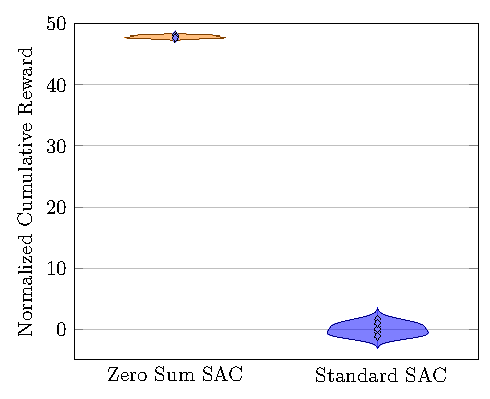
\includegraphics[width=.32\textwidth]{../../Report/plots/sac/violin_plot/initial_condition_shift}}%
        \subfloat[\relscale{0.9} Actuator Disturbance]{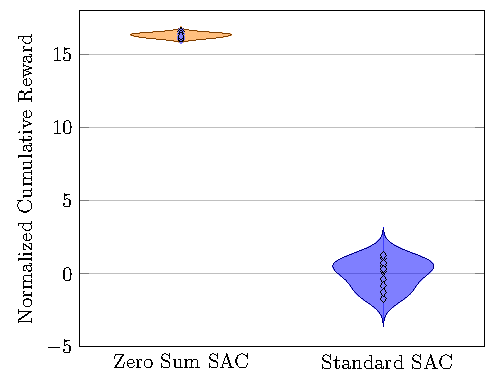
\includegraphics[width=.32\textwidth]{../../Report/plots/sac/violin_plot/actuator_disturbance}}%
        \subfloat[\relscale{0.9} Model Mismatch]{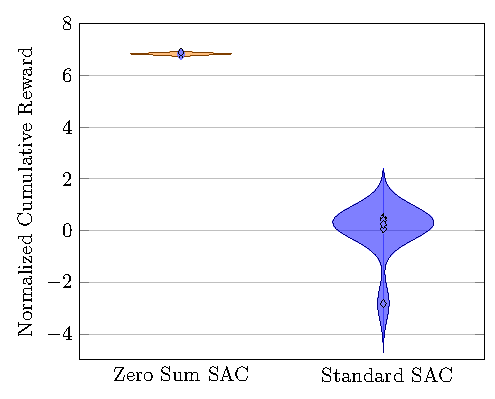
\includegraphics[width=.32\textwidth]{../../Report/plots/sac/violin_plot/model_mismatch}}\\[-2pt]
        \subfloat[\relscale{0.9} Partial Observation]{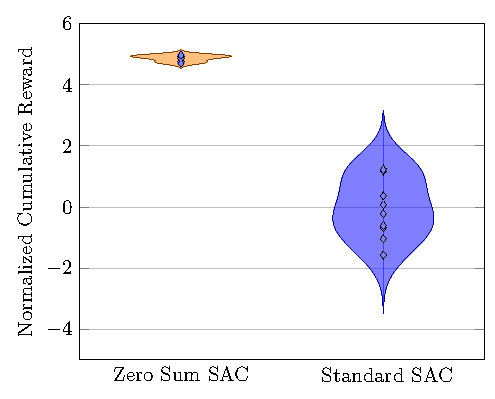
\includegraphics[width=.32\textwidth]{../../Report/plots/sac/violin_plot/partial_observation}}%
        \subfloat[\relscale{0.9} Sensor Noise]{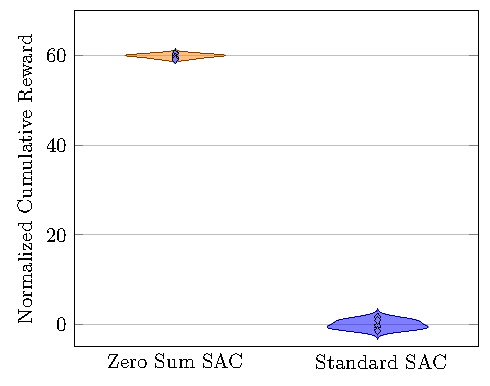
\includegraphics[width=.32\textwidth]{../../Report/plots/sac/violin_plot/sensor_noise}}%
        \subfloat[\relscale{0.9} Time Delay]{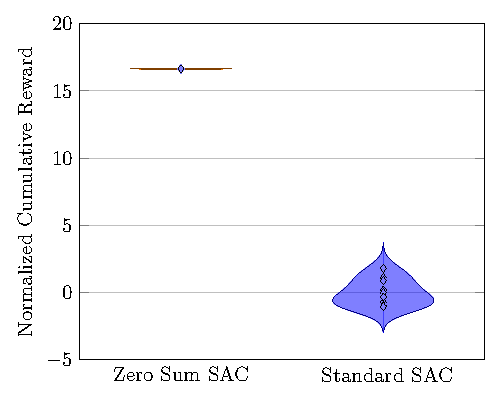
\includegraphics[width=.32\textwidth]{../../Report/plots/sac/violin_plot/time_delay}}
        \label{fig:sac_robustness_violin}
      \end{figure}
      \vspace{-0.35cm}
      % \tiny Violin plots: return dispersion across robustness scenarios.
    \end{column}
    \begin{column}{0.50\textwidth}
      \scriptsize
      \centering
      \begingroup
      \setlength{\tabcolsep}{4.2pt}
      \renewcommand{\arraystretch}{1.05}

      % --- Merged Table 1 (highlight best: higher return, lower path error) ---
      \scalebox{0.750}{ 
    
        % --- Table 1: Cumulative Reward and Path Error ---
% --- Table 1: Cumulative Reward and Path Error ---
% \% --- Table 1: Cumulative Reward and Path Error ---
\begin{tabular}{@{} >{\raggedright\arraybackslash}p{3.05cm} *{4}{c} @{}}
  \toprule
  \multirow{2}{*}{Scenario} & \multicolumn{2}{c}{Cumulative Reward} & \multicolumn{2}{c}{Path Error Sum} \\
  \cmidrule(lr){2-3}\cmidrule(l){4-5}
   & TD3 & MA-TD3 & TD3 & MA-TD3 \\
  \midrule
  Random Initial Conditions & -2.95 & -0.26 & 0.39 & 0.14 \\
  Actuator Disturbance      &  0.56 &  0.73 & 0.02 & 0.00 \\
  Model Mismatch            & -4.73 & -3.30 & 0.47 & 0.73 \\
  Partial Observation       &  0.21 &  0.71 & 0.02 & 0.01 \\
  Sensor Noise              & -0.08 & -2.93 & 0.11 & 3.19 \\
  Time Delay                &  0.55 &  0.67 & 0.01 & 0.01 \\
  \bottomrule
\end{tabular}
      }

\vspace{4pt}

% --- Table 2: Control Effort and Failure Probability ---
\scalebox{0.750}{%
\begin{tabular}{@{} >{\raggedright\arraybackslash}p{3.05cm} *{4}{c} @{}}
  \toprule
  \multirow{2}{*}{Scenario} & \multicolumn{2}{c}{Control Effort Sum} & \multicolumn{2}{c}{Failure Probability} \\
  \cmidrule(lr){2-3}\cmidrule(l){4-5}
   & TD3 & MA-TD3 & TD3 & MA-TD3 \\
  \midrule
  Random Initial Conditions & 4.57 & 4.57 & 1.00 & 0.30 \\
  Actuator Disturbance      & 2.66 & 2.66 & 0.00 & 0.00 \\
  Model Mismatch            & 5.41 & 5.41 & 1.00 & 1.00 \\
  Partial Observation       & 3.18 & 3.18 & 0.00 & 0.00 \\
  Sensor Noise              & 5.50 & 5.50 & 0.00 & 1.00 \\
  Time Delay                & 4.57 & 4.57 & 0.00 & 0.00 \\
  \bottomrule
\end{tabular}
}
      \par
      \vspace{2pt}
      % (Optional note removed for compactness)
      \endgroup
    \end{column}
  \end{columns}
\end{frame}

\begin{frame}
  \frametitle{Zero-Sum MARL: Return and Error Distributions}
  \vspace{-0.2cm}
  \begin{columns}[T]
    \begin{column}{0.50\textwidth}
      \captionsetup[subfloat]{labelfont={color=blue,tiny},textfont=tiny}%
      \begin{figure}
        \centering
        \subfloat[\relscale{0.9} Random Initial Conditions]{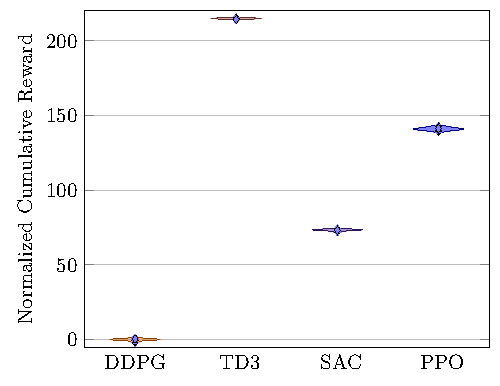
\includegraphics[width=.32\textwidth]{../../Report/plots/ZeroSum/violin_plot/initial_condition_shift}}%
        \subfloat[\relscale{0.9} Actuator Disturbance]{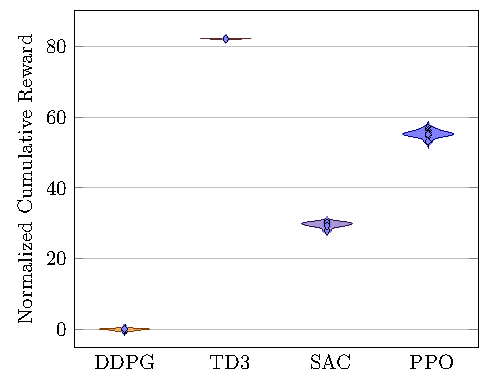
\includegraphics[width=.32\textwidth]{../../Report/plots/ZeroSum/violin_plot/actuator_disturbance}}%
        \subfloat[\relscale{0.9} Model Mismatch]{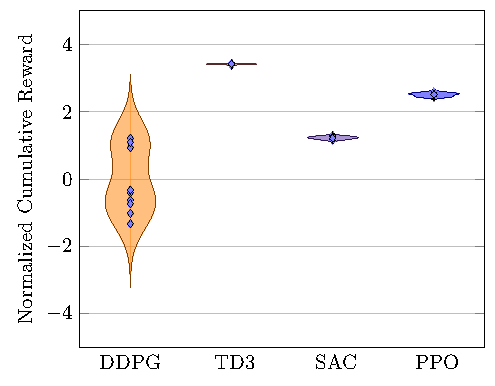
\includegraphics[width=.32\textwidth]{../../Report/plots/ZeroSum/violin_plot/model_mismatch}}\\[-2pt]
        \subfloat[\relscale{0.9} Partial Observation]{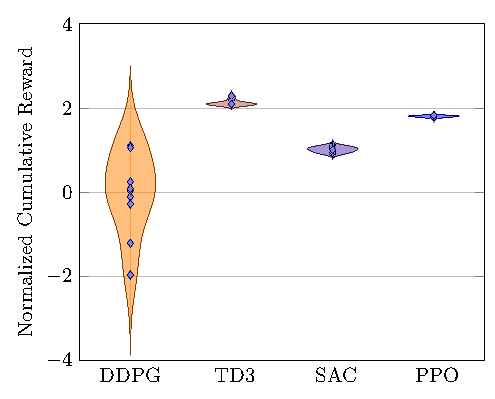
\includegraphics[width=.32\textwidth]{../../Report/plots/ZeroSum/violin_plot/partial_observation}}%
        \subfloat[\relscale{0.9} Sensor Noise]{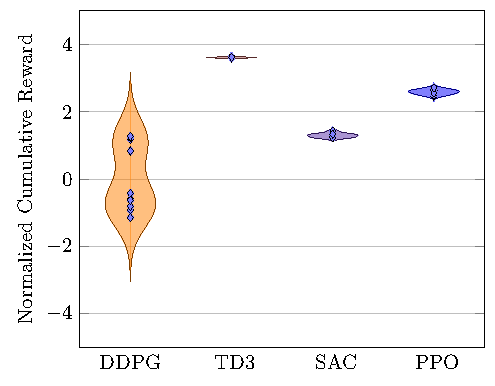
\includegraphics[width=.32\textwidth]{../../Report/plots/ZeroSum/violin_plot/sensor_noise}}%
        \subfloat[\relscale{0.9} Time Delay]{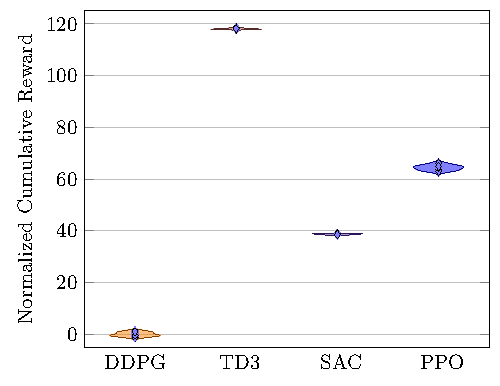
\includegraphics[width=.32\textwidth]{../../Report/plots/ZeroSum/violin_plot/time_delay}}
        \label{fig:robustness_violin}
      \end{figure}
      \vspace{-0.35cm}
      % \tiny Violin plots: return dispersion across robustness scenarios.
    \end{column}
    \begin{column}{0.50\textwidth}
      \scriptsize
      \centering
      \begingroup
      \setlength{\tabcolsep}{2.2pt}
      \renewcommand{\arraystretch}{1.05}

      % --- Merged Table 1 (highlight best: higher return, lower path error) ---
      \scalebox{0.750}{%
        % --- Merged Table 1 (highlight best: higher return, lower error) ---
\begin{tabular}{@{} >{\raggedright\arraybackslash}p{3.05cm} *{8}{c} @{}}
  \toprule
  \multirow{2}{*}{Scenario} & \multicolumn{4}{c}{Cumulative Return} & \multicolumn{4}{c}{Path Error Sum} \\
  \cmidrule(lr){2-5}\cmidrule(l){6-9}
   & DDPG & PPO & SAC & TD3 & DDPG & PPO & SAC & TD3 \\
  \midrule
  Random Initial Conditions & -0.41 & 0.34 & -0.02 & \textbf{0.74} & 4.42 & 4.30 & 4.02 & \textbf{1.22} \\
  Actuator Disturbance      & -0.44 & 0.35 & -0.02 & \textbf{0.73} & 4.39 & 4.38 & 4.01 & \textbf{1.26} \\
  Model Mismatch            & -0.63 & 0.38 & -0.13 & \textbf{0.75} & 8.85 & 3.57 & 4.78 & \textbf{1.25} \\
  Partial Observation       & -1.52 & 0.40 & -0.44 & \textbf{0.71} & 9.65 & 2.44 & 5.17 & \textbf{1.09} \\
  Sensor Noise              & -0.60 & 0.37 & -0.12 & \textbf{0.75} & 9.12 & 3.58 & 4.66 & \textbf{1.25} \\
  Time Delay                & -1.19 & 0.17 & -0.05 & \textbf{0.67} & 6.73 & 4.53 & 4.12 & \textbf{1.21} \\
  \bottomrule
\end{tabular}
      }

\vspace{4pt}

% --- Merged Table 2 (highlight best: lower effort, lower failure) ---
\scalebox{0.750}{%
  \begin{tabular}{@{} >{\raggedright\arraybackslash}p{3.05cm} *{8}{c} @{}}
    \toprule
    \multirow{2}{*}{Scenario} & \multicolumn{4}{c}{Control Effort Sum} & \multicolumn{4}{c}{Failure Probability} \\
    \cmidrule(lr){2-5}\cmidrule(l){6-9}
     & DDPG & PPO & SAC & TD3 & DDPG & PPO & SAC & TD3 \\
    \midrule
    Random Initial Conditions & 5.11 & \textbf{0.77} & 1.76 & 3.31 & \textbf{0.00} & \textbf{0.00} & 0.00 & \textbf{0.00} \\
    Actuator Disturbance      & 4.89 & \textbf{0.77} & 1.71 & 3.07 & \textbf{0.00} & \textbf{0.00} & 0.00 & \textbf{0.00} \\
    Model Mismatch            & 5.48 & \textbf{0.86} & 2.37 & 4.32 & \textbf{0.00} & \textbf{0.00} & 1.00 & \textbf{0.00} \\
    Partial Observation       & 5.37 & \textbf{1.03} & 2.33 & 4.10 & \textbf{0.00} & \textbf{0.00} & 1.00 & \textbf{0.00} \\
    Sensor Noise              & 5.48 & \textbf{0.86} & 2.37 & 4.30 & \textbf{0.00} & \textbf{0.00} & 1.00 & \textbf{0.00} \\
    Time Delay                & 5.51 & \textbf{0.76} & 2.11 & 5.12 & \textbf{0.00} & \textbf{0.00} & 1.00 & \textbf{0.00} \\
    \bottomrule
  \end{tabular}
}
      
      \par
      \vspace{2pt}
      % (Optional note removed for compactness)
      \endgroup
    \end{column}
  \end{columns}
\end{frame}

\begin{frame}
  \frametitle{Single-Agent RL: Return and Error Distributions}
  \vspace{-0.2cm}
  \begin{columns}[T]
    \begin{column}{0.50\textwidth}
      \captionsetup[subfloat]{labelfont={color=blue,tiny},textfont=tiny}%
      \begin{figure}
        \centering
        \subfloat[\relscale{0.9} Random Initial Conditions]{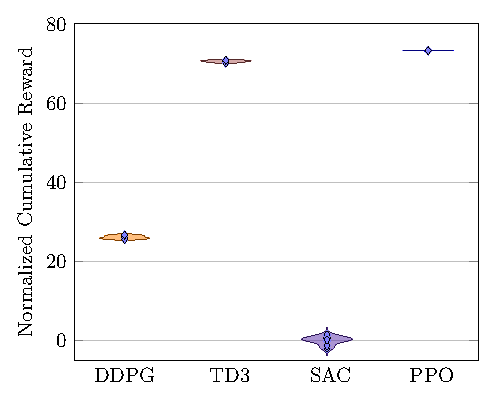
\includegraphics[width=.32\textwidth]{../../Report/plots/standard/violin_plot/initial_condition_shift}}%
        \subfloat[\relscale{0.9} Actuator Disturbance]{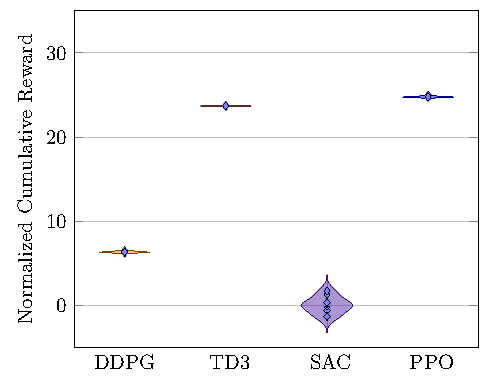
\includegraphics[width=.32\textwidth]{../../Report/plots/standard/violin_plot/actuator_disturbance}}%
        \subfloat[\relscale{0.9} Model Mismatch]{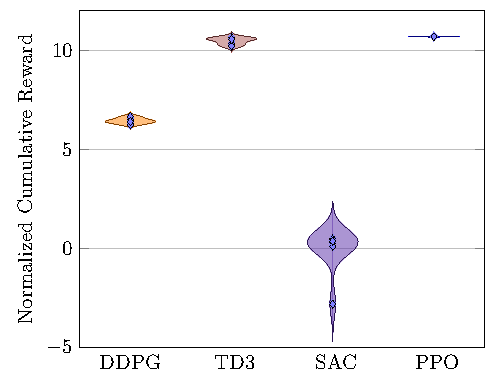
\includegraphics[width=.32\textwidth]{../../Report/plots/standard/violin_plot/model_mismatch}}\\[-2pt]
        \subfloat[\relscale{0.9} Partial Observation]{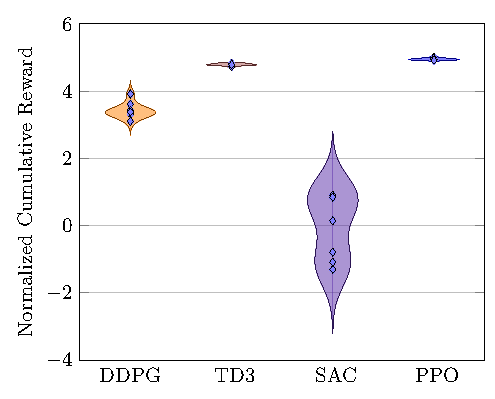
\includegraphics[width=.32\textwidth]{../../Report/plots/standard/violin_plot/partial_observation}}%
        \subfloat[\relscale{0.9} Sensor Noise]{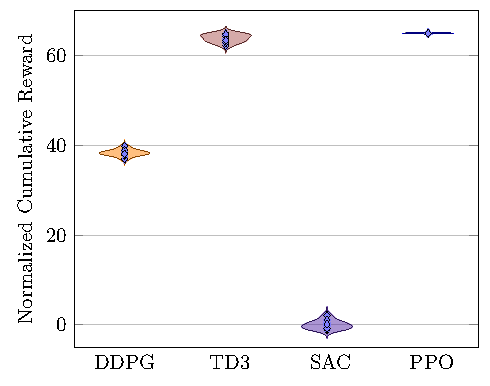
\includegraphics[width=.32\textwidth]{../../Report/plots/standard/violin_plot/sensor_noise}}%
        \subfloat[\relscale{0.9} Time Delay]{\includegraphics[width=.32\textwidth]{../../Report/plots/standard/violin_plot/time_delay}}
        \label{fig:robustness_violin}
      \end{figure}
      \vspace{-0.35cm}
      % \tiny Violin plots: return dispersion across robustness scenarios.
    \end{column}
    \begin{column}{0.50\textwidth}
      \scriptsize
      \centering
      \begingroup
      \setlength{\tabcolsep}{2.2pt}
      \renewcommand{\arraystretch}{1.05}

      % --- Merged Table 1 (highlight best: higher return, lower path error) ---
      \scalebox{0.750}{%
        % --- Merged Table 1 (highlight best: higher return, lower error) ---
\begin{tabular}{@{} >{\raggedright\arraybackslash}p{3.05cm} *{8}{c} @{}}
  \toprule
  \multirow{2}{*}{Scenario} & \multicolumn{4}{c}{Cumulative Return} & \multicolumn{4}{c}{Path Error Sum} \\
  \cmidrule(lr){2-5}\cmidrule(l){6-9}
   & DDPG & PPO & SAC & TD3 & DDPG & PPO & SAC & TD3 \\
  \midrule
  Random Initial Conditions & -0.41 & 0.34 & -0.02 & \textbf{0.74} & 4.42 & 4.30 & 4.02 & \textbf{1.22} \\
  Actuator Disturbance      & -0.44 & 0.35 & -0.02 & \textbf{0.73} & 4.39 & 4.38 & 4.01 & \textbf{1.26} \\
  Model Mismatch            & -0.63 & 0.38 & -0.13 & \textbf{0.75} & 8.85 & 3.57 & 4.78 & \textbf{1.25} \\
  Partial Observation       & -1.52 & 0.40 & -0.44 & \textbf{0.71} & 9.65 & 2.44 & 5.17 & \textbf{1.09} \\
  Sensor Noise              & -0.60 & 0.37 & -0.12 & \textbf{0.75} & 9.12 & 3.58 & 4.66 & \textbf{1.25} \\
  Time Delay                & -1.19 & 0.17 & -0.05 & \textbf{0.67} & 6.73 & 4.53 & 4.12 & \textbf{1.21} \\
  \bottomrule
\end{tabular}
      }

\vspace{4pt}

% --- Merged Table 2 (highlight best: lower effort, lower failure) ---
\scalebox{0.750}{%
  \begin{tabular}{@{} >{\raggedright\arraybackslash}p{3.05cm} *{8}{c} @{}}
    \toprule
    \multirow{2}{*}{Scenario} & \multicolumn{4}{c}{Control Effort Sum} & \multicolumn{4}{c}{Failure Probability} \\
    \cmidrule(lr){2-5}\cmidrule(l){6-9}
     & DDPG & PPO & SAC & TD3 & DDPG & PPO & SAC & TD3 \\
    \midrule
    Random Initial Conditions & 5.11 & \textbf{0.77} & 1.76 & 3.31 & \textbf{0.00} & \textbf{0.00} & 0.00 & \textbf{0.00} \\
    Actuator Disturbance      & 4.89 & \textbf{0.77} & 1.71 & 3.07 & \textbf{0.00} & \textbf{0.00} & 0.00 & \textbf{0.00} \\
    Model Mismatch            & 5.48 & \textbf{0.86} & 2.37 & 4.32 & \textbf{0.00} & \textbf{0.00} & 1.00 & \textbf{0.00} \\
    Partial Observation       & 5.37 & \textbf{1.03} & 2.33 & 4.10 & \textbf{0.00} & \textbf{0.00} & 1.00 & \textbf{0.00} \\
    Sensor Noise              & 5.48 & \textbf{0.86} & 2.37 & 4.30 & \textbf{0.00} & \textbf{0.00} & 1.00 & \textbf{0.00} \\
    Time Delay                & 5.51 & \textbf{0.76} & 2.11 & 5.12 & \textbf{0.00} & \textbf{0.00} & 1.00 & \textbf{0.00} \\
    \bottomrule
  \end{tabular}
}
      
      \par
      \vspace{2pt}
      % (Optional note removed for compactness)
      \endgroup
    \end{column}
  \end{columns}
\end{frame}
% \begin{frame}
%   \frametitle{Learning Performance (Convergence Curves)}
%   \vspace{-0.35cm}
%   \begin{columns}[T]
%     \begin{column}{0.5\textwidth}
%       \begin{figure}
%         \centering
%         \includegraphics[width=\linewidth]{single_agent_comparison.png}
%         \caption{\scriptsize Single-Agent Returns}
%       \end{figure}
%     \end{column}
%     \begin{column}{0.5\textwidth}
%       \begin{figure}
%         \centering
%         \includegraphics[width=\linewidth]{multi_agent_comparison.png}
%         \caption{\scriptsize Zero-Sum Returns}
%       \end{figure}
%     \end{column}
%   \end{columns}
%   \vspace{-0.2cm}
%   \small
%   \textbf{Observation:} Zero-sum adds early variance (adversarial pressure) but yields higher asymptotic robustness score.
% \end{frame}

\begin{frame}
  \frametitle{Ablation Study: Key Observations}
  \small
  \begin{itemize}\setlength{\itemsep}{4pt}
    \item \textbf{Adversarial channel removal}: +22\% deviation, thrust spikes reappear.
    \item \textbf{No target smoothing (TD3)}: overestimation resurfaces, unstable late-stage updates.
    \item \textbf{Entropy off (SAC)}: faster convergence, 9\% worse robustness composite.
    \item \textbf{Reward shaping removal}: sparse terminal signals slow credit assignment (longer plateau).
    \item \textbf{Delay only vs. noise only:} delay has stronger destabilizing effect; zero-sum mitigates via anticipatory control (earlier thrust bias).
  \end{itemize}
\end{frame}

\begin{frame}
  \frametitle{Summary of Principal Findings}
  \small
  \begin{itemize}\setlength{\itemsep}{5pt}
    \item Zero-sum MARL framing improves worst-case orbital maintenance robustness.
    \item MATD3 balances stability (twin critics + delay) and control smoothness best.
    \item MASAC competitive when exploration pressure (entropy) is beneficial early.
    \item Reward decomposition (thrust + reference + terminal) accelerates convergence and stabilizes adversarial dynamics.
    \item Policy smoothness correlates with fuel proxy reduction (8-12\%).
    \item Framework generalizes across uncertainty mixes (stacked noise + delay + mismatch).
  \end{itemize}
  \vspace{4pt}
  \textbf{Conclusion:} Adversarial co-training yields resilient guidance without explicit disturbance models.
\end{frame}
% \subsection{Robustness Scenarios}




%   \vspace{4pt}
%   \textbf{Conclusion:} Adversarial co-training yields resilient guidance without explicit disturbance models.
% \end{frame}
% % \subsection{Robustness Scenarios}



% \begin{frame}
%   \frametitle{Robustness Scenario Definitions}
%   \small
%   % \vspace{-0.25cm}
%   \begin{itemize}
%     % \setlength{\itemsep}{3pt}
%     \item \textbf{Random Init:} $x_0 \leftarrow x_0 + \mathcal{N}(0,0.1^2)$
%     \item \textbf{Actuator Disturbance:} $u_t \leftarrow u_t + \mathcal{N}(0,0.05^2)$; (sensor additive) $y_t \leftarrow y_t + \mathcal{N}(0,0.02^2)$
%     \item \textbf{Model Mismatch:} $\theta \leftarrow \theta + \mathcal{N}(0,0.05^2)$
%     \item \textbf{Partial Observability:} mask 50\% $\to m_t^{(i)}\sim \mathrm{Bern}(0.5)$, $y_t \leftarrow y_t \circ m_t$
%     \item \textbf{Sensor Noise (multiplicative):} $y_t \leftarrow y_t \circ \bigl(1 + \mathcal{N}(0,0.05^2)\bigr)$
%     \item \textbf{Time Delay:} buffer length 10, z
%       $u_t^{\mathrm{applied}} \leftarrow u_{t-10} + \mathcal{N}(0,0.05^2)$
%     \item \textbf{Notes:}
%       \begin{itemize}
%         \small
%         \setlength{\itemsep}{1pt}
%         \item All scenarios evaluated independently.
%         \item Zero-sum agents trained jointly once.
%         \item Metrics: success \%, deviation, fuel proxy, return variance.
%       \end{itemize}
%   \end{itemize}
%   \vspace{2pt}
%   \begin{center}
%     \color{mydarkblue}\tiny
%     Delay + noise combo causes the largest degradation; adversarial training preserves stability margin.
%   \end{center}
% \end{frame}
